\documentclass[conference]{IEEEtran}

% Packages (kept consistent with provided template)
\usepackage{graphicx}
\usepackage{amsmath}
\usepackage{url}
\usepackage{fancyhdr}
\usepackage{color}
\usepackage{hyperref}
\usepackage{subcaption}
\usepackage{booktabs}
\usepackage{siunitx}
\usepackage{listings}

\definecolor{headergray}{gray}{0.6}
\addtolength{\topmargin}{10pt}

% Listings (Python snippets)
\lstset{
  basicstyle=\ttfamily\footnotesize,
  breaklines=true,
  frame=single,
  columns=fullflexible,
  language=Python,
  showstringspaces=false
}

\title{Semantic Segmentation on Cityscapes with DeepLabV3+}

\author{%
\IEEEauthorblockN{Francesco Albano}
\IEEEauthorblockA{%
Student ID: LJ2506219\\
School of Computer Science\\
Beihang University (BUAA)\\
Beijing, China\\
Email: francescoalbano@buaa.edu.cn, francescoalbano357@gmail.com
}}

\begin{document}

\pagestyle{fancy}
\fancyhead[C]{\textcolor{headergray}{Final Project – Student ID: LJ2506219 – Artificial Intelligence}}
\renewcommand{\headrulewidth}{0pt}
\fancyfoot[C]{\thepage}
\setlength{\footskip}{40pt}

\maketitle

\begin{abstract}
This report describes the implementation and evaluation of a semantic segmentation pipeline on the Cityscapes dataset using a DeepLabV3+ architecture. The project includes an end-to-end training script configurable from the command line, a robust checkpointing system enabling interruption and exact resumption of training, and utilities to generate predictions compliant with the official Cityscapes submission format. Development and early experiments were conducted on macOS (CPU/MPS) for rapid iteration, while full training was executed on Google Colab using an NVIDIA T4 GPU. This not only significantly reduced training time, but also enabled higher model quality by allowing for larger batch sizes, longer training schedules, and more extensive experimentation compared to CPU/MPS.
\end{abstract}

\begin{IEEEkeywords}
Semantic segmentation, Cityscapes, DeepLabV3+, PyTorch, data augmentation, checkpointing, cosine annealing, evaluation server
\end{IEEEkeywords}

\section{Introduction}
\label{sec:introduction}
Semantic segmentation assigns a semantic label to every pixel in an image, enabling fine-grained scene understanding for applications such as autonomous driving, robotics, and intelligent transportation systems. Cityscapes is a widely used benchmark for urban street scenes, providing high-resolution images and dense pixel annotations for both validation and test evaluation through an official server. The goal of this project is to train a segmentation model capable of producing Cityscapes-compliant predictions and to document the complete experimental pipeline, from data loading and augmentation to checkpoint management and quantitative evaluation.

\section{Design and Implementation}
\label{sec:design}
This section describes the implemented pipeline by following the project codebase structure.

\subsection{Project Structure and Entry Points}
The project exposes three main command-line entry points:
\begin{itemize}
\item \texttt{train.py}: training, evaluation, and visualization modes via a unified CLI.
\item \texttt{evaluate.py}: evaluation on the validation set given a checkpoint.
\item \texttt{generate\_cityscapes\_predictions.py}: generation of predictions in the official Cityscapes submission format.
\end{itemize}
All scripts build on a common module layout under \texttt{src/}: data loading (\texttt{src/data}), model definition (\texttt{src/models}), training (\texttt{src/training}), evaluation metrics (\texttt{src/evaluation}), and visualization utilities (\texttt{src/utils}).

In addition, the project provides a Jupyter notebook (\texttt{analyze\_checkpoints.ipynb}) specifically designed to analyze all saved checkpoints and extract training metrics. This utility was used to generate the summary statistics and plots reported in the results and appendix sections.

\subsection{Model Architecture: DeepLabV3+}
The implemented model is DeepLabV3+ with a ResNet-50 encoder. The code constructs an encoder-decoder architecture with:
\begin{itemize}
\item A ResNet backbone split into stages (\texttt{layer0}--\texttt{layer4}).
\item An Atrous Spatial Pyramid Pooling (ASPP) module applied on deep features to aggregate multi-scale context.
\item A decoder branch that fuses ASPP features with low-level features (from an earlier backbone stage) and upsamples to the input resolution.
\end{itemize}
The final output is a dense logit tensor at the original input resolution, enabling per-pixel classification.

\subsection{Data Loading and Label Mapping}
Two dataset access patterns are available:
\begin{itemize}
\item A wrapper around \texttt{torchvision.datasets.Cityscapes} (\texttt{CityscapesDataset}) primarily used for inference/submission generation where filenames are needed.
\item A custom raw-file loader (\texttt{CityscapesRawDataset}) designed to apply Albumentations transforms in a coordinated way to both the image and the segmentation mask.
\end{itemize}

Cityscapes provides multiple label encodings. The training pipeline targets the standard 19-class \textit{trainId} setting, and uses \texttt{ignore\_index=255} for void/unlabeled pixels.

\subsection{Data Augmentation and Preprocessing}
By default, the training dataloaders use Albumentations transforms to apply geometric and photometric augmentations consistently to image and mask:
\begin{itemize}
\item resize to the training resolution,
\item random scaling and random cropping to the target size,
\item horizontal flipping,
\item color jitter and brightness/contrast perturbations,
\item optional Gaussian blur,
\item normalization using ImageNet mean and standard deviation.
\end{itemize}
Validation uses only deterministic resizing and normalization, avoiding any stochastic augmentation.

\subsection{Loss Function and Optimization}
The main training loss is pixel-wise cross entropy with an ignore index:
\begin{equation}
\mathcal{L}_{CE} = - \sum_{c=1}^{C} y_c \log p_c, \quad \text{with ignored pixels excluded.}
\end{equation}
Class weighting is supported but disabled in the reported training configuration. The optimizer is AdamW with parameter groups that allow assigning different learning rates to backbone and head parameters. In particular, the backbone group uses a smaller learning rate than the decoder/head, reflecting standard fine-tuning practice.

\subsection{Learning Rate Scheduling: Cosine Annealing}
The training code supports either a polynomial schedule or cosine annealing. The reported experiment uses cosine annealing with a minimum learning rate $\eta_{min}$. In its standard form, cosine annealing updates the learning rate as:
The polynomial schedule reduces the learning rate following a power law, typically as $\eta(t) = \eta_{max} (1 - t/T)^{p}$, where $t$ is the current step, $T$ is the total number of steps, and $p$ is the power. This results in a smooth, monotonic decay of the learning rate. Cosine annealing, instead, decreases the learning rate following a cosine curve, periodically allowing for larger learning rates and potentially helping the optimizer escape local minima.
\begin{equation}
\eta(t) = \eta_{min} + \frac{1}{2}(\eta_{max}-\eta_{min})\left(1+\cos\left(\pi \frac{t}{T}\right)\right),
\end{equation}
where $T$ is the schedule horizon.

\subsection{Training Configuration via Command Line}
Training is controlled through a single script with explicit command-line arguments. The following configuration was used for the GPU run on Google Colab:
\begin{lstlisting}
python train.py \
  --architecture deeplabv3plus \
  --image-size 512 1024 \
  --batch-size 8 \
  --learning-rate 3e-4 \
  --weight-decay 1e-4 \
  --num-epochs 60 \
  --scheduler cosine \
  --min-lr 1e-6 \
  --no-class-weights \
  --no-weighted-sampler \
  --device cuda
\end{lstlisting}
This approach is beneficial because it (i) exposes the main hyperparameters, (ii) enables systematic experimentation by changing a small set of flags, and (iii) adapts seamlessly to different hardware backends (CPU/MPS for development, CUDA for full training).

\subsection{Hardware and Execution Environment}
Early development and sanity checks were executed on macOS using CPU/MPS to speed up iteration and debugging. Full training was then moved to Google Colab and executed on an NVIDIA T4 GPU, which not only substantially reduces training time compared to CPU/MPS, but also enables higher model quality by supporting larger batch sizes, longer training, and more complex experiments that would not be feasible on CPU/MPS.

\subsection{Checkpointing and Robust Resume}
A full checkpoint is saved after each epoch. Each checkpoint contains:
\begin{itemize}
\item model parameters,
\item optimizer state,
\item AMP scaler state (when applicable),
\item epoch index,
\item training history (losses and validation metrics),
\item training image resolution.
\end{itemize}

This enables the training to be interrupted at any time and resumed exactly from the next epoch. As a demonstrative case, training was:
\begin{itemize}
\item executed up to epoch 13,
\item interrupted,
\item resumed from the saved checkpoint,
\item continued from epoch 14 to epoch 25 without further interruptions.
\end{itemize}
This scenario demonstrates robustness of the checkpointing design and does not represent a limitation of the method.

\subsection{Evaluation and Cityscapes Submission}
Cityscapes evaluation is typically performed via an official server, especially for the test split where ground truth annotations are not publicly available. For this reason, the project includes a dedicated script that generates predictions in the required format:
\begin{itemize}
\item predictions are computed as per-pixel argmax over class logits,
\item outputs are resized to the original Cityscapes resolution (2048\,$\times$\,1024) using nearest-neighbor interpolation,
\item predictions are converted from \textit{trainId} to the official \textit{id} labels,
\item files are saved with the naming convention \texttt{*\_gtFine\_labelIds.png}.
\end{itemize}
This step is essential to ensure compatibility with the Cityscapes benchmark and to obtain standardized metrics from the official evaluation pipeline.

\section{Results}
\label{sec:results}
This section reports quantitative results based exclusively on the checkpoint analysis output contained in \texttt{checkpoint\_results.yaml}.


\subsection{Checkpoint Metrics (Epoch 1--25)}
Table~\ref{tab:checkpoint_summary} summarizes representative checkpoints.
All metrics (loss, pixel accuracy, mIoU) are available for every checkpoint and their evolution across epochs is visualized in the summary plots at the end of the report (Figures~\ref{fig:loss_curves} and~\ref{fig:miou_curve}). In the table below, we show a selection of representative checkpoints: epochs 13 and 14 are included to demonstrate the interruption and successful resume from a checkpoint, while epochs 24 and 25 correspond respectively to the best validation mIoU and the final epoch. This selection highlights both the robustness of the checkpointing system and the model's best performance.

\begin{table}[ht]
\centering
\caption{Representative checkpoint metrics extracted from \texttt{checkpoint\_results.yaml}.}
\label{tab:checkpoint_summary}
\begin{tabular}{@{}ccccc@{}}
	oprule
Epoch & Train Loss & Val Loss & Pixel Acc. & mIoU \\
\midrule
1  & 0.5826 & 0.3557 & 0.8831 & 0.2923 \\
13 & 0.1830 & 0.1883 & 0.9364 & 0.4330 \\
14 & 0.1797 & 0.1901 & 0.9366 & 0.4412 \\
24 & 0.1468 & 0.1746 & 0.9423 & 0.4574 \\
25 & 0.1458 & 0.1797 & 0.9410 & 0.4397 \\
\bottomrule
\end{tabular}
\end{table}

\subsection{Performance Evolution}
From epoch 1 to epoch 13, the model shows a clear improvement across all metrics: training loss decreases from 0.5826 to 0.1830, while validation mIoU increases from 0.2923 to 0.4330. After resuming training (epoch 14 onward), performance continues to improve and reaches its best reported validation mIoU at epoch 24 (0.4574) with a pixel accuracy of 0.9423. A slight drop is observed at epoch 25 (mIoU 0.4397), indicating that validation performance may fluctuate in late epochs even as training loss keeps decreasing.



\section{Testing and Validation}
\label{sec:testing}
Testing focused on both correctness and usability:
\begin{itemize}
\item Environment verification: a dedicated setup script checks imports, PyTorch backend availability (CPU/MPS/CUDA), model construction, transforms, and label mapping.
\item Training sanity checks: short runs on macOS (CPU/MPS) validate the end-to-end pipeline before moving to GPU training.
\item Metric validation: evaluation uses pixel accuracy and mean IoU with an ignore index, ensuring void pixels do not bias results.
\item Checkpoint robustness: interruption and resume were validated by restoring optimizer state and continuing from a later epoch.
\end{itemize}

\section{User Guide}
\label{sec:user_guide}
This section describes how to reproduce the main project steps.

\subsection{Training}
Run training with the desired configuration:
\begin{lstlisting}
python train.py \
  --mode train \
  --data-root ./data/cityscapes \
  --architecture deeplabv3plus \
  --image-size 512 1024 \
  --batch-size 8 \
  --learning-rate 3e-4 \
  --weight-decay 1e-4 \
  --num-epochs 60 \
  --scheduler cosine \
  --min-lr 1e-6 \
  --no-class-weights \
  --no-weighted-sampler \
  --device cuda
\end{lstlisting}
To resume from a checkpoint:
\begin{lstlisting}
python train.py \
  --mode train \
  --data-root ./data/cityscapes \
  --load-checkpoint ./checkpoints/checkpoint_epoch_13.pth \
  --device cuda
\end{lstlisting}

\subsection{Evaluation}
Evaluate a trained checkpoint on the validation set:
\begin{lstlisting}
python evaluate.py \
  --checkpoint ./checkpoints/best_model.pth \
  --device cuda
\end{lstlisting}

\subsection{Generating Cityscapes-Format Predictions (Submission)}
Generate predictions and prepare the submission zip:
\begin{lstlisting}
python generate_cityscapes_predictions.py \
  --checkpoint ./checkpoints/best_model.pth \
  --data-root ./data/cityscapes \
  --split val \
  --output-dir ./cityscapes_results \
  --device cuda

cd cityscapes_results
zip -r ../cityscapes_predictions.zip .
\end{lstlisting}
The resulting archive can be uploaded to the Cityscapes evaluation server.

\subsection{Qualitative Visualizations (Overlay Examples)}
To visually assess the quality of the model's predictions, you can generate overlay images that combine the original input with the predicted segmentation mask. This allows for an intuitive evaluation of how well the model distinguishes different classes and scene elements.

You can use the provided visualization or inference utilities to create these overlays. For example, to generate an overlay for a single image, run:
\begin{lstlisting}
python inference.py \
  --image path/to/leftImg8bit.png \
  --checkpoint ./checkpoints/best_model.pth \
  --device cuda \
  --output overlay_example.png
\end{lstlisting}
This will save an image with the predicted segmentation overlaid on the original. Example overlays are included in the appendix.

\section{Conclusion}
\label{sec:conclusion}
This project implements an end-to-end semantic segmentation workflow for Cityscapes using DeepLabV3+. The system provides a configurable training interface, robust checkpointing and resumption, and tooling for producing Cityscapes-compliant prediction files for official evaluation. Quantitative results extracted from the checkpoint analysis show consistent improvement across epochs, reaching a best validation mIoU of 0.4574 at epoch 24, with pixel accuracy of 0.9423. The combination of a GPU training environment and a resumable training pipeline supports efficient experimentation while maintaining reproducibility.

Despite the solid performance, the achieved mIoU is lower than state-of-the-art results on Cityscapes, mainly due to limited training epochs, the use of a ResNet-50 backbone (pretrained on ImageNet only), and the absence of additional large-scale pretraining beyond ImageNet. Future work could therefore focus on longer training schedules, stronger backbones (e.g., ResNet-101 or transformer-based models), and enhanced pretraining or semi-supervised strategies.

\section{Open Source Availability}
\label{sec:open_source}
The project repository is available at: \url{https://github.com/fra2404/segmentation-cityscape}

\section*{Acknowledgment}
This project was developed as the final project for the Artificial Intelligence course at Beihang University (BUAA).

\begin{thebibliography}{99}

\bibitem{cityscapes}
M. Cordts et al., ``The Cityscapes Dataset for Semantic Urban Scene Understanding,'' \emph{CVPR}, 2016.

\bibitem{deeplabv3plus}
L.-C. Chen et al., ``Encoder-Decoder with Atrous Separable Convolution for Semantic Image Segmentation,'' \emph{ECCV}, 2018.

\bibitem{adamw}
I. Loshchilov and F. Hutter, ``Decoupled Weight Decay Regularization,'' \emph{ICLR}, 2019.

\bibitem{albumentations}
A. Buslaev et al., ``Albumentations: Fast and Flexible Image Augmentations,'' \emph{Information}, 2020.

\bibitem{duda}
R. O. Duda, P. E. Hart, and D. G. Stork, \emph{Pattern Classification}, 2nd ed. New York, NY, USA: Wiley-Interscience, 2001. (Course textbook)

\end{thebibliography}

\clearpage
\onecolumn
\appendix

\section{Figures: Training Curves}
\label{sec:appendix_curves}
This section presents the main training curves that summarize the quantitative evolution of the model during training. The following figures show the progression of training and validation loss, as well as the mean Intersection over Union (mIoU) metric on the validation set, across all epochs. These plots provide insight into the model's learning dynamics, convergence behavior, and generalization performance. 

To obtain these results, all training checkpoints were systematically analyzed using the provided \texttt{analyze\_checkpoints.ipynb} notebook. This process generated the \texttt{checkpoint\_results.yaml} file, which records the metrics for each checkpoint and enables detailed tracking of the model's progress throughout training. The two plots below separately show the evolution of loss (training and validation) and validation mIoU, based on this comprehensive analysis as discussed in Section~\ref{sec:results}.

\begin{figure}[ht]
\centering
\IfFileExists{loss_curves.png}{%
  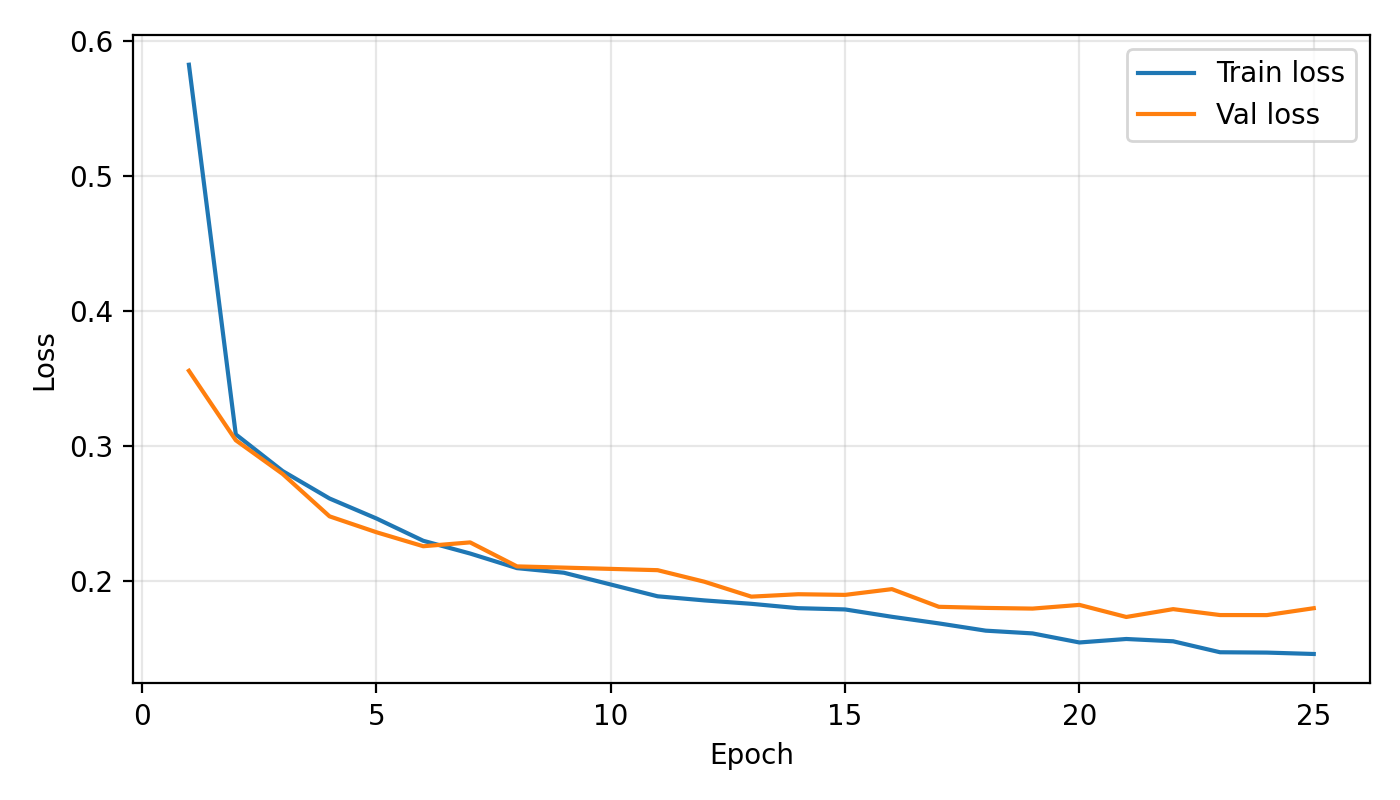
\includegraphics[width=0.8\textwidth]{loss_curves.png}%
}{%
  \fbox{\parbox{0.8\textwidth}{\centering Placeholder: loss\_curves.png (generate using the provided plotting utility script).}}%
}
\caption{Training and validation loss curves (generated from \texttt{checkpoint\_results.yaml}).}
\label{fig:loss_curves}
\end{figure}

\begin{figure}[ht]
\centering
\IfFileExists{miou_curve.png}{%
  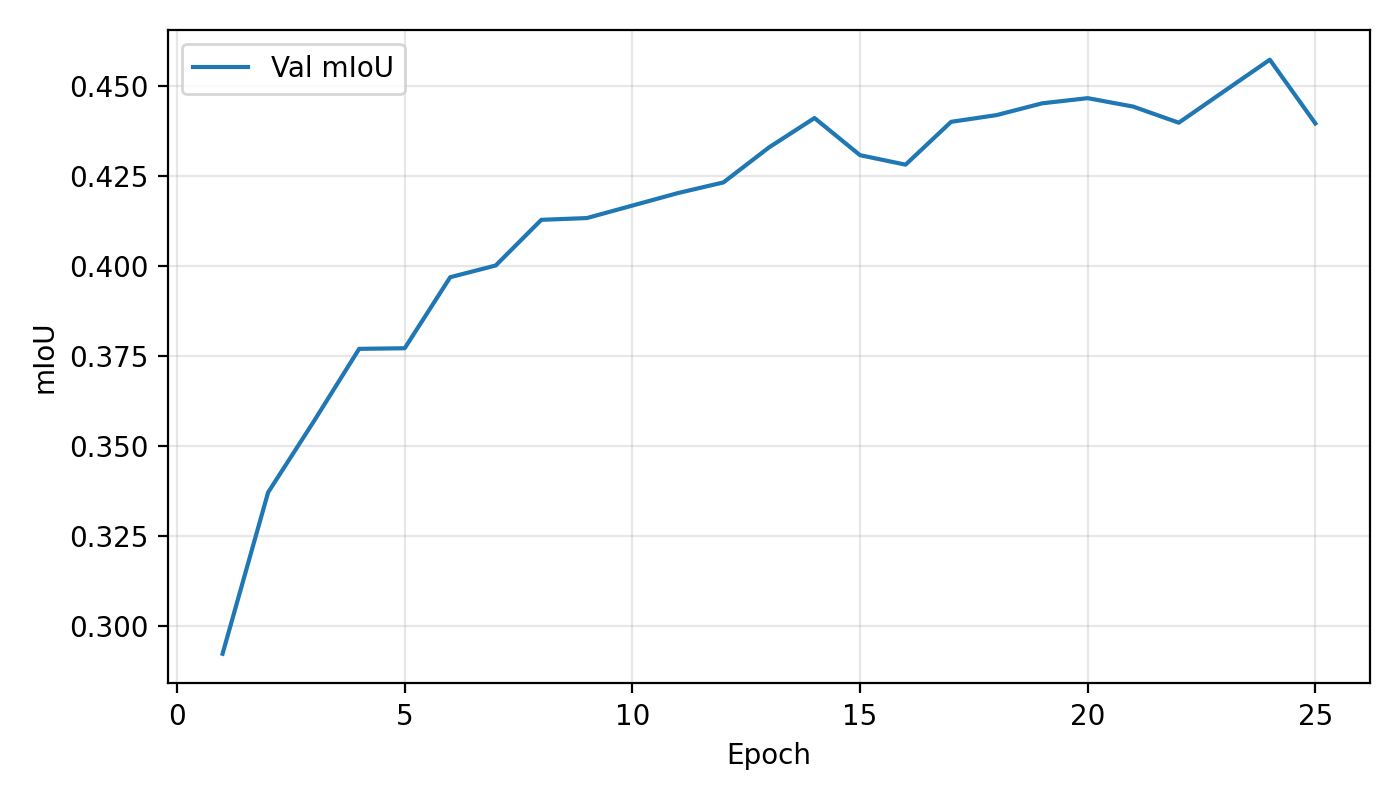
\includegraphics[width=0.8\textwidth]{miou_curve.png}%
}{%
  \fbox{\parbox{0.9\textwidth}{\centering Placeholder: miou\_curve.png (generate using the provided plotting utility script).}}%
}
\caption{Validation mIoU over epochs (generated from \texttt{checkpoint\_results.yaml}).}
\label{fig:miou_curve}
\end{figure}

\clearpage
\section{Figures: Qualitative Overlay Examples}
\label{sec:appendix_overlays}

For compactness and diversity, the following overlays include images from different Cityscapes cities (e.g., Frankfurt, Münster) to show the model's behavior on various urban scenes. To further test generalization, two additional overlays are shown for external images (downloaded from the internet, not present in the training set). This allows qualitative assessment both on in-distribution and out-of-distribution data.

The overlays below correspond to:
\begin{itemize}
  \item Three validation images from Frankfurt (Cityscapes val split)
  \item One validation image from Münster (Cityscapes val split)
  \item Two external photos (test.webp and pexels-joshsorenson-139303.jpg) downloaded from the web
\end{itemize}


% Frankfurt overlays
\begin{figure}[ht]
\centering
\IfFileExists{images/overlay_example_1.png}{%
  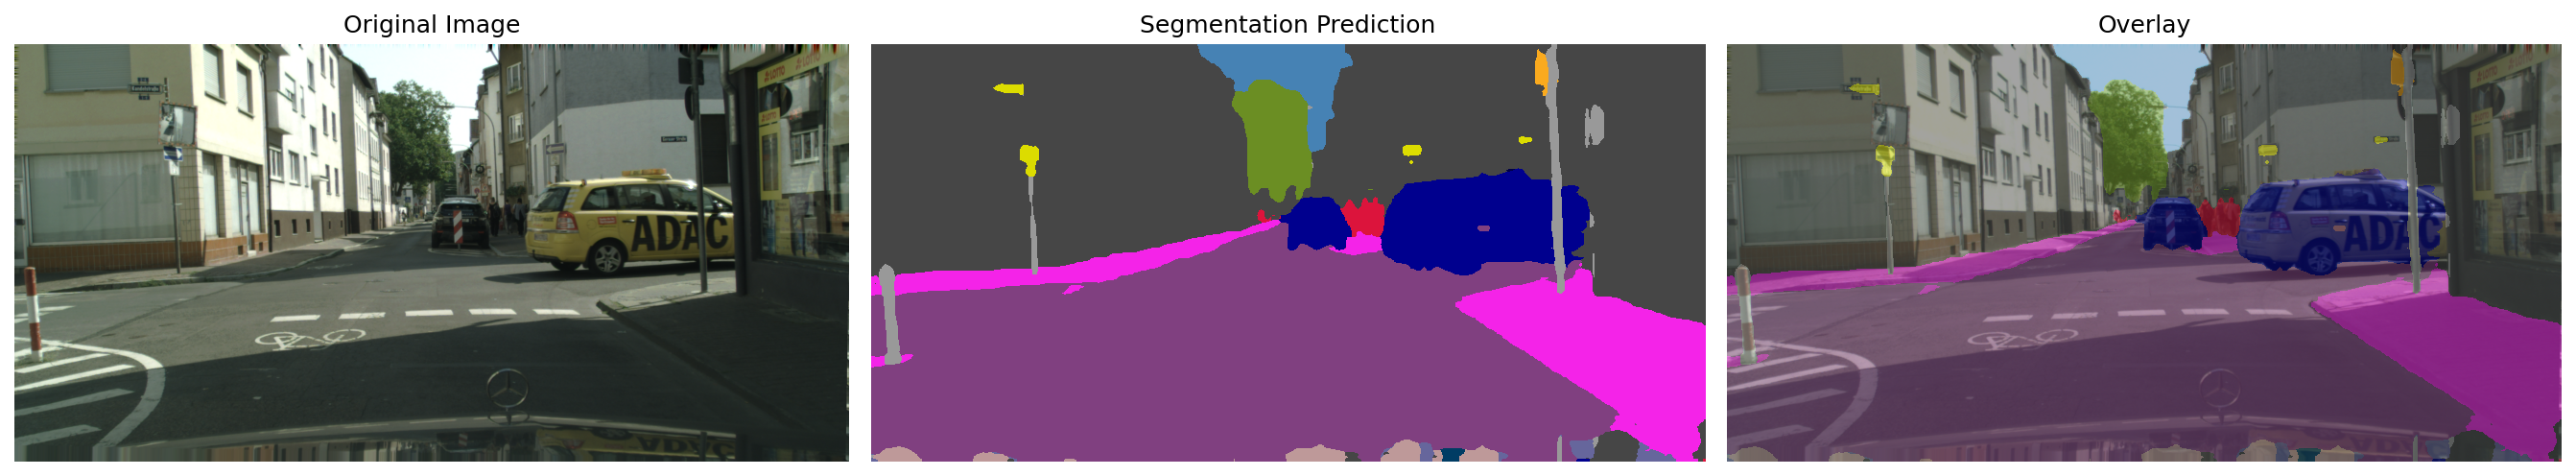
\includegraphics[width=0.9\textwidth]{images/overlay_example_1.png}%
}{%
  \fbox{\parbox{0.9\textwidth}{\centering Placeholder: overlay\_example\_1.png (export an overlay with inference/visualization utilities).}}%
}
\caption{Overlay example 1: Cityscapes val, Frankfurt.}
\label{fig:overlay1}
\end{figure}

\begin{figure}[ht]
\centering
\IfFileExists{images/overlay_example_2.png}{%
  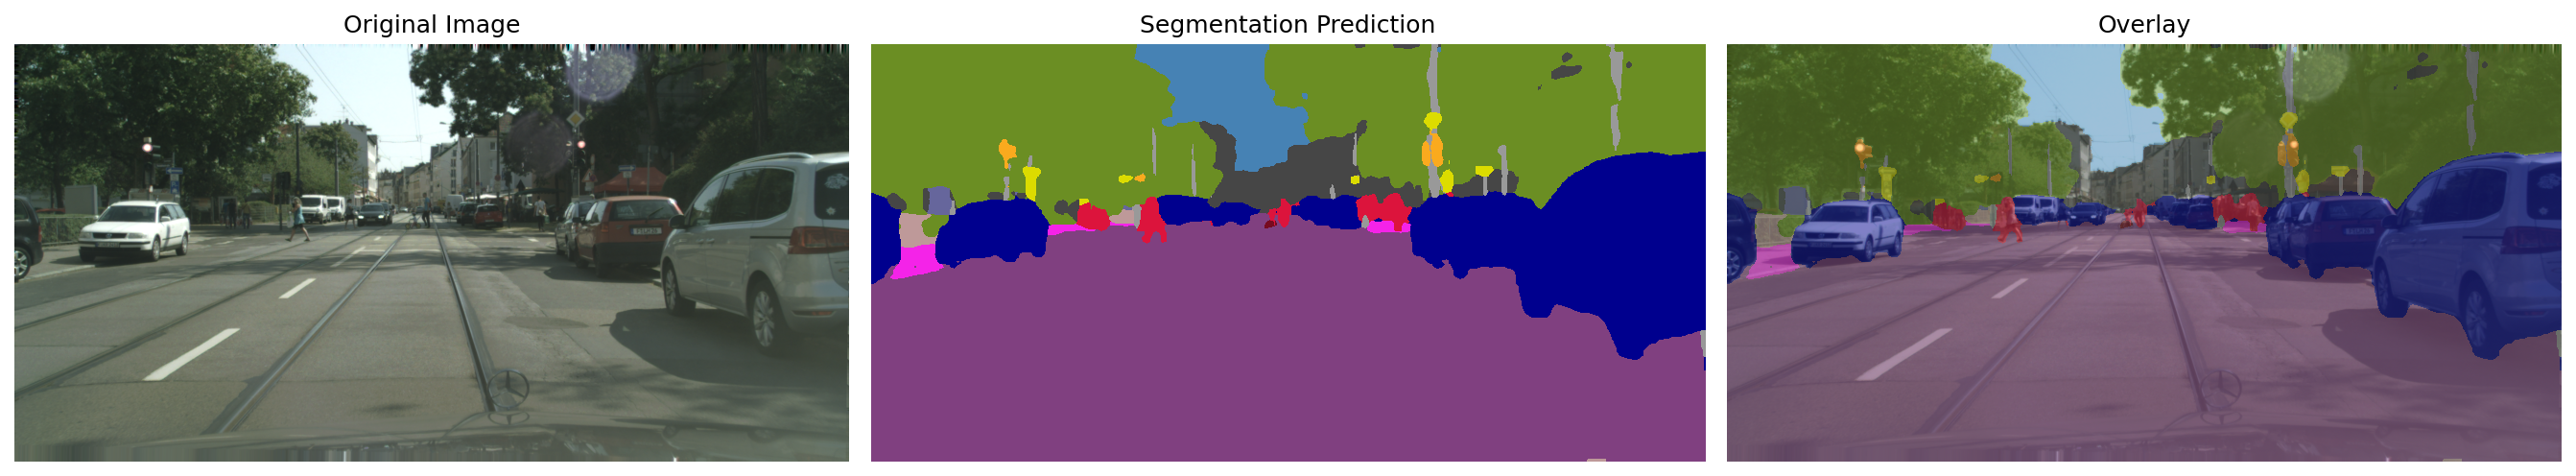
\includegraphics[width=0.9\textwidth]{images/overlay_example_2.png}%
}{%
  \fbox{\parbox{0.9\textwidth}{\centering Placeholder: overlay\_example\_2.png (export an overlay with inference/visualization utilities).}}%
}
\caption{Overlay example 2: Cityscapes val, Frankfurt.}
\label{fig:overlay2}
\end{figure}

\begin{figure}[ht]
\centering
\IfFileExists{images/overlay_example_3.png}{%
  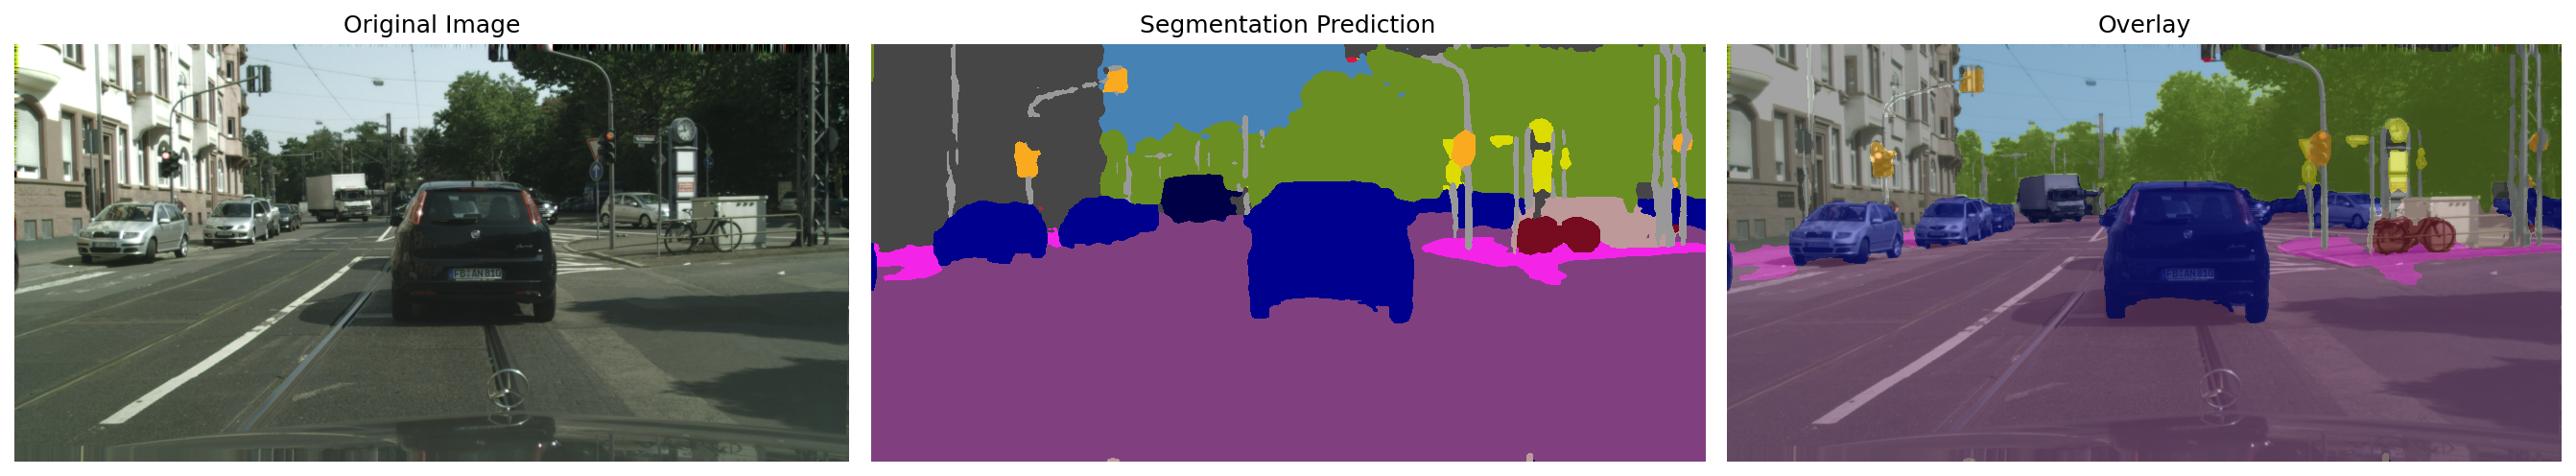
\includegraphics[width=0.9\textwidth]{images/overlay_example_3.png}%
}{%
  \fbox{\parbox{0.9\textwidth}{\centering Placeholder: overlay\_example\_3.png (export an overlay with inference/visualization utilities).}}%
}
\caption{Overlay example 3: Cityscapes val, Frankfurt.}
\label{fig:overlay3}
\end{figure}

% Munster overlay
\begin{figure}[ht]
\centering
\IfFileExists{images/overlay_example_munster.png}{%
  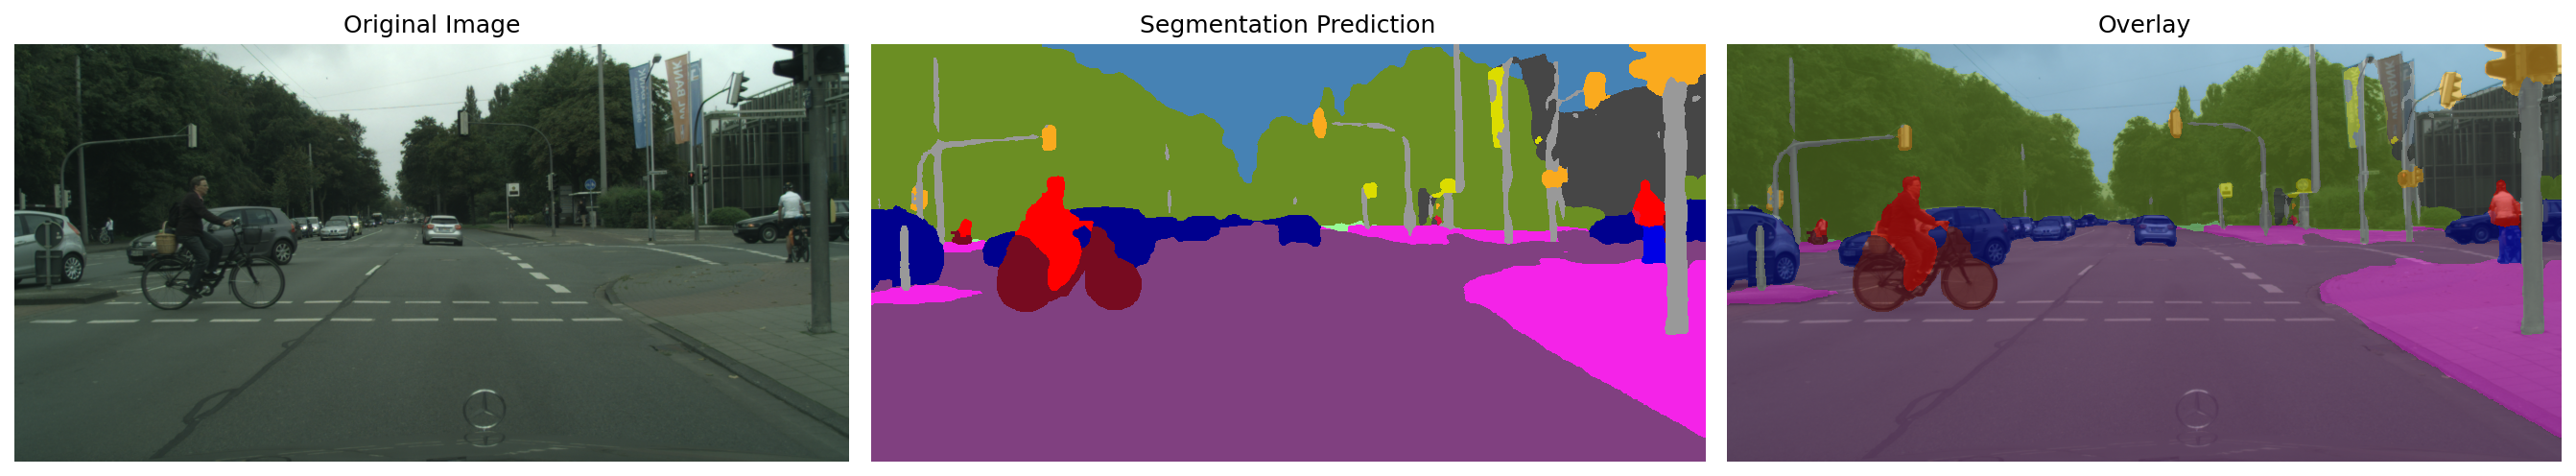
\includegraphics[width=0.9\textwidth]{images/overlay_example_munster.png}%
}{%
  \fbox{\parbox{0.9\textwidth}{\centering Placeholder: overlay\_example\_munster.png (export an overlay with inference/visualization utilities).}}%
}
\caption{Overlay example 4: Cityscapes val, Münster.}
\label{fig:overlay_munster}
\end{figure}

% External image overlay
\begin{figure}[ht]
\centering
\IfFileExists{images/overlay_example_test.png}{%
  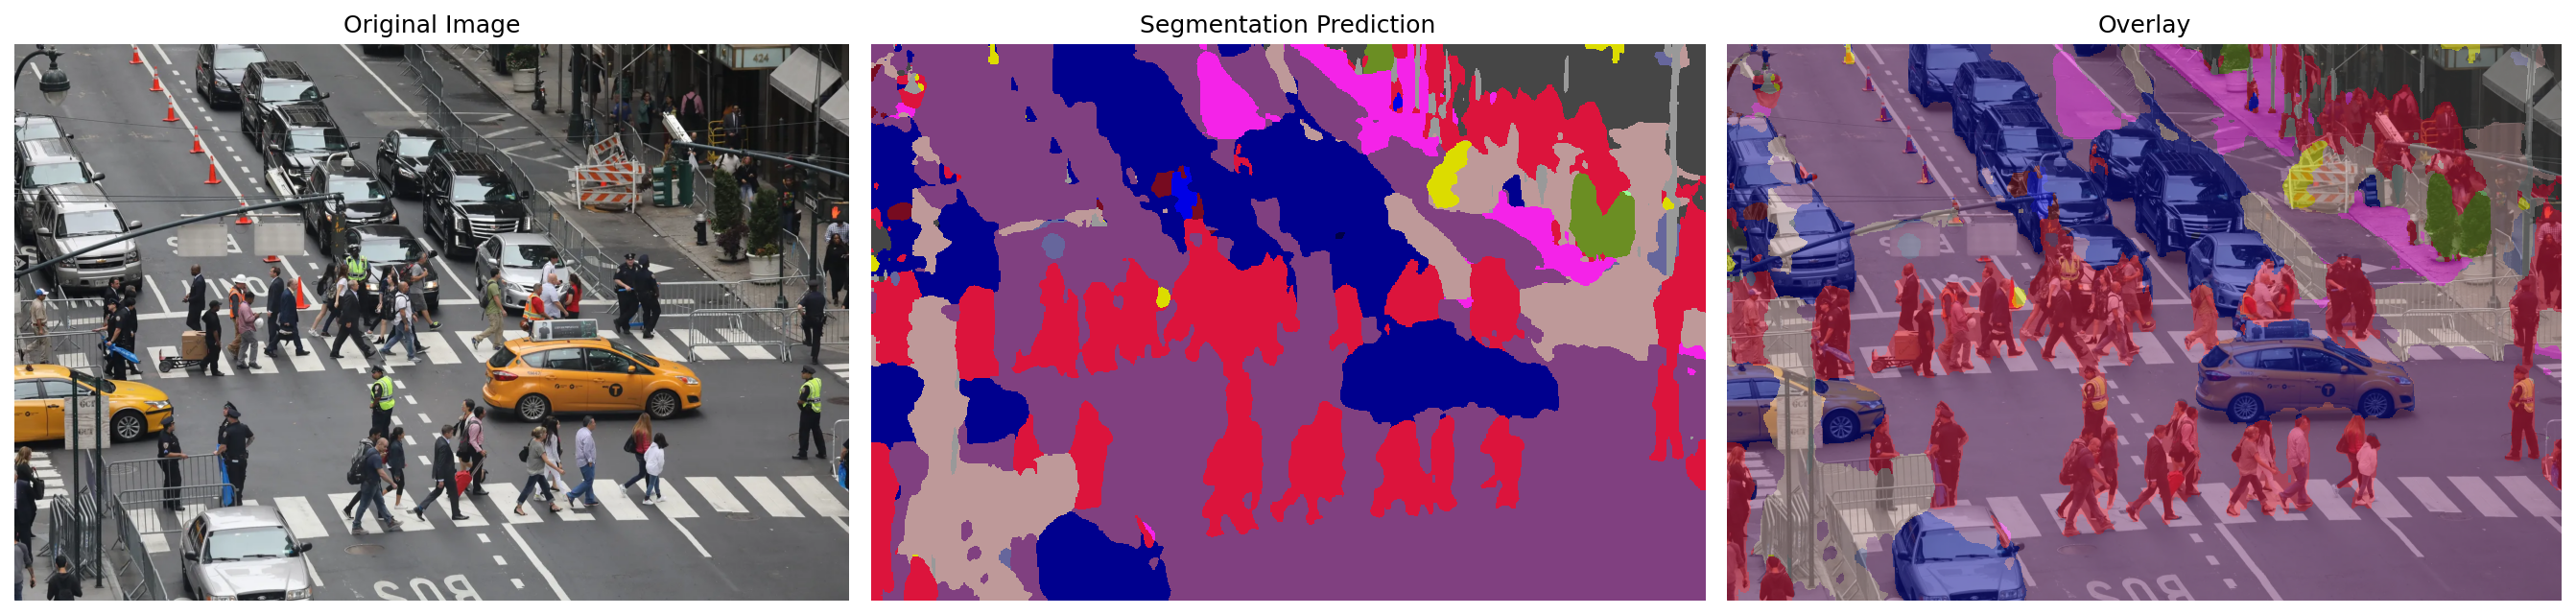
\includegraphics[width=0.9\textwidth]{images/overlay_example_test.png}%
}{%
  \fbox{\parbox{0.9\textwidth}{\centering Placeholder: overlay\_example\_test.png (export an overlay with inference/visualization utilities).}}%
}

\caption{Overlay example 5: external image (test.webp) downloaded from the web.}
\label{fig:overlay_test}
\end{figure}

% Second external image overlay
\begin{figure}[ht]
\centering
\IfFileExists{images/overlay_example_test2.png}{%
  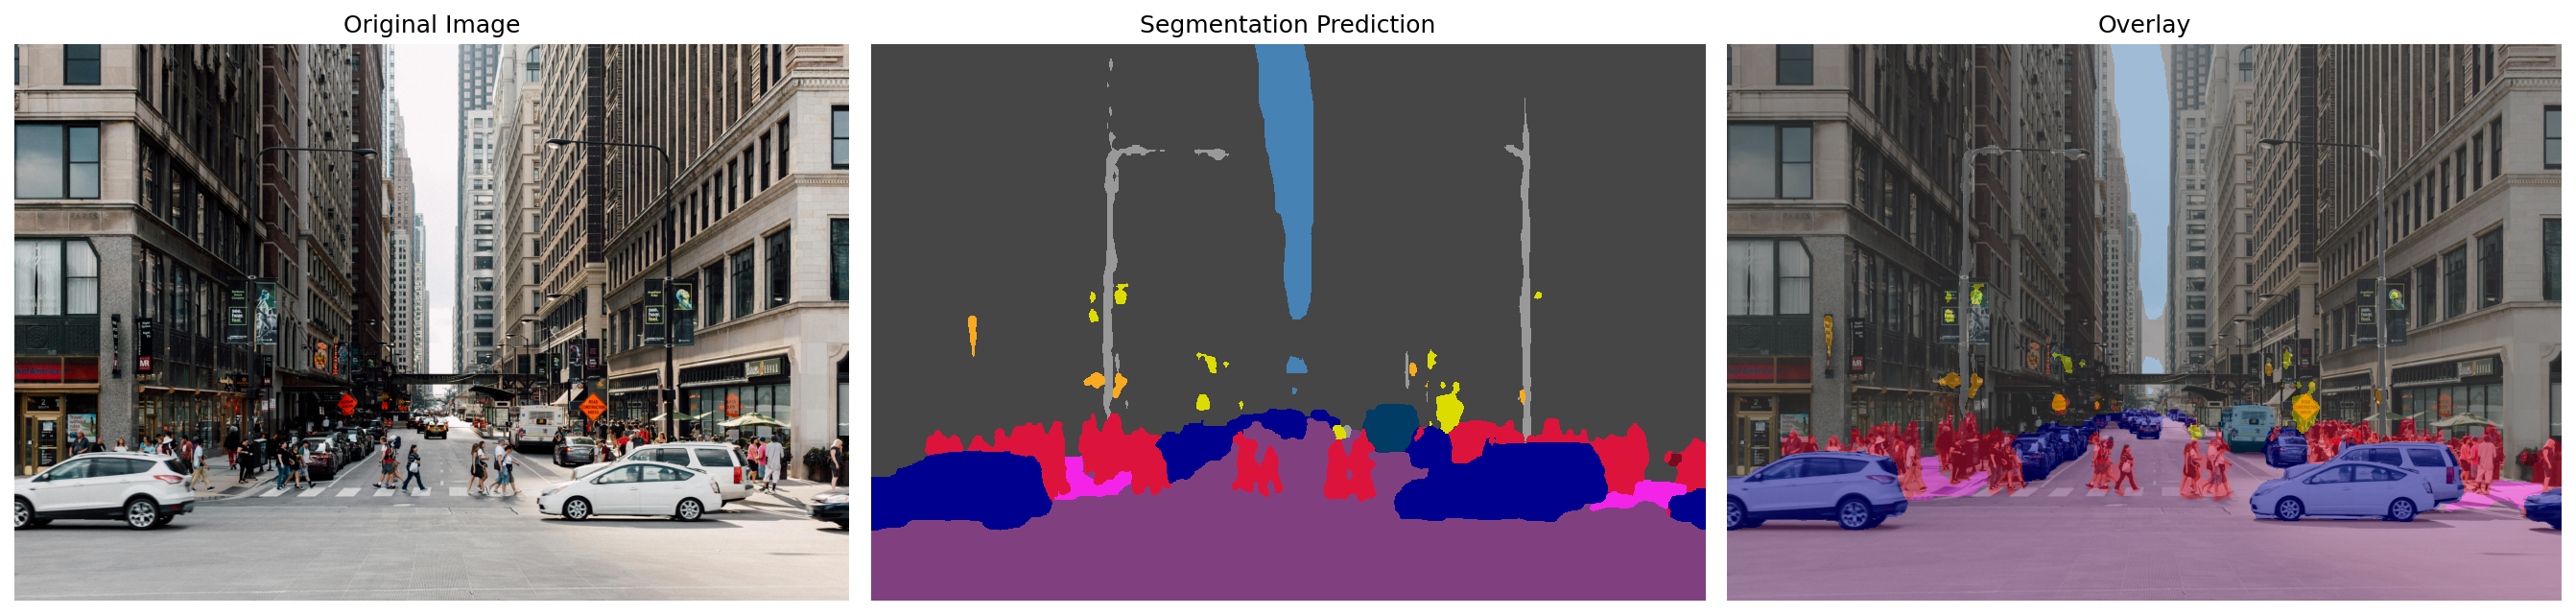
\includegraphics[width=0.9\textwidth]{images/overlay_example_test2.png}%
}{%
  \fbox{\parbox{0.9\textwidth}{\centering Placeholder: overlay\_example\_test2.png (export an overlay with inference/visualization utilities).}}%
}
\caption{Overlay example 6: external image (pexels-joshsorenson-139303.jpg) downloaded from the web.}
\label{fig:overlay_test2}
\end{figure}

\end{document}
